\chapter{El modelo de transporte}\label{cap:modelo}

\section{Zonas y red}

El territorio se divide en $Z=12$ zonas: nueve de Bogotá, que agrupan las veinte localidades por
contigüidad y por el corredor que las sirve, y tres de la región (Soacha, Sabana Occidente y Sabana
Norte). La \cref{tab:zonas} presenta su población en 2025, la deriva anual de su demanda y su
participación en la atracción de viajes. Las poblaciones de Suba, Kennedy, Soacha y de los municipios
principales provienen de \citet{dane2025}; las demás son aproximaciones del autor que suman el total
oficial de Bogotá y están documentadas en el archivo \texttt{datos/zonas.csv}.

\begin{table}[ht]
\centering\small
\caption{Zonas del modelo: población 2025, deriva de la demanda ($\mu_i$, demografía más la tendencia
común de 0,5\,\% anual), volatilidad idiosincrática ($s_i$) y participación en la atracción.}\label{tab:zonas}
\resizebox{\textwidth}{!}{\begin{tabular}{lllrrrr}
\toprule
Código & Zona & Ámbito & Población (miles) & $\mu_i$ & $s_i$ & Atracción \\
\midrule
CEN & Centro ampliado & Bogotá & 512 & -0,3\,\% & 3\,\% & 30,0\,\% \\
USA & Usaquén & Bogotá & 545 & 0,0\,\% & 3\,\% & 9,0\,\% \\
SUB & Suba & Bogotá & 1.246 & 0,5\,\% & 3\,\% & 8,0\,\% \\
ENG & Engativá – Barrios Unidos & Bogotá & 1.000 & -0,1\,\% & 3\,\% & 9,0\,\% \\
FON & Fontibón – Puente Aranda & Bogotá & 670 & 0,4\,\% & 3\,\% & 13,0\,\% \\
KEN & Kennedy & Bogotá & 1.080 & 0,1\,\% & 3\,\% & 8,0\,\% \\
BOS & Bosa & Bogotá & 760 & 1,1\,\% & 3\,\% & 3,5\,\% \\
SOC & Suroccidente & Bogotá & 1.320 & 0,9\,\% & 3\,\% & 4,0\,\% \\
SOR & Suroriente & Bogotá & 805 & -0,1\,\% & 3\,\% & 4,5\,\% \\
SOA & Soacha & Región & 870 & 1,7\,\% & 4\,\% & 3,0\,\% \\
SAO & Sabana Occidente & Región & 560 & 2,5\,\% & 4\,\% & 4,0\,\% \\
SAN & Sabana Norte & Región & 610 & 2,3\,\% & 4\,\% & 4,0\,\% \\
\bottomrule
\end{tabular}
}
\fuente{DANE (2025), Encuesta Multipropósito 2025 y aproximaciones del autor.}
\end{table}

La red tiene $E=18$ corredores (\cref{fig:red}): once radiales hacia el centro ampliado, cinco
transversales del anillo occidental (avenidas 68, Boyacá y Ciudad de Cali) y dos conexiones
periféricas. Cada corredor representa el conjunto de vías paralelas que sirven una misma relación y se
modela en ambos sentidos, de modo que el grafo dirigido tiene $D=36$ arcos. La longitud de cada
corredor es la distancia geodésica entre los centroides multiplicada por un factor de circuidad de
1,3.

\begin{figure}[ht]
\centering
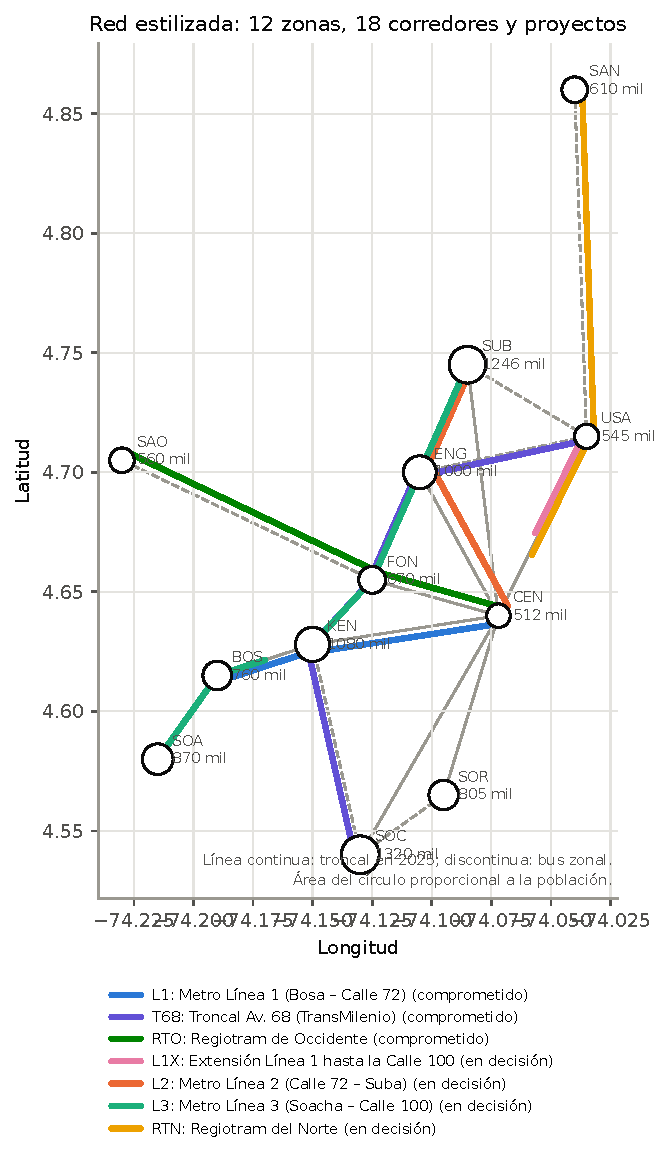
\includegraphics[height=.72\textheight]{figuras/fig_red.pdf}
\caption{Red estilizada: zonas (área proporcional a la población), corredores y proyectos.}\label{fig:red}
\end{figure}

\paragraph{Oferta de transporte público.} Cada corredor tiene una oferta de transporte público (TP)
formada por servicios $s$ con capacidad $C_s$ (pasajeros por hora y sentido), velocidad $v_s$ y
fracción cubierta del corredor $\phi_s$: el servicio base (troncal de TransMilenio a 25,2 km/h o bus
zonal a 15 km/h) y los proyectos abiertos. El tiempo en vehículo por kilómetro es la media armónica
ponderada por capacidad,
\begin{equation}\label{eq:armonica}
h_e=\frac{1}{K_e}\sum_{s\in e}\frac{C_s\phi_s}{v_s},\qquad K_e=\sum_{s\in e}C_s\phi_s,
\end{equation}
y $K_e$ es la capacidad total del corredor.

\section{Demanda}

\subsection{Generación}

En la hora pico de la mañana se generan $V_0=\ViajesPicoBase$ mil viajes motorizados en el año base,
que equivalen al 10\,\% de los viajes diarios en TP, automóvil, motocicleta y taxi según la encuesta de
2023. La generación de la zona $i$ en el año $t$ y el escenario $\omega$ es
\begin{equation}\label{eq:generacion}
P_i(t,\omega)=V_0\,g_i\,X_i(t,\omega)\,\big(1-\kappa\,\theta\,r(t)\big),
\end{equation}
donde $g_i$ es la participación de la zona (proporcional a su población, con una tasa de 0,85 para los
municipios), $X_i$ es el índice de demanda del MBG, $\theta$ la intensidad de la política de suelo,
$\kappa$ la fracción máxima de viajes motorizados que pasan a modos no motorizados y $r(t)$ la rampa
lineal de implementación entre 2027 y 2040.

\subsection{Política de proximidad y policentrismo}\label{sec:suelo}

La política tiene dos efectos. El primero está en \eqref{eq:generacion}: con $\theta=1$, el
$\kappa=5\,\%$ de los viajes motorizados se hace a pie o en bicicleta al final de la rampa; esos viajes
no desaparecen del costo social, sino que se cargan con 20 minutos de tiempo no motorizado. El segundo
es la relocalización de una fracción $\rho\theta r(t)$ de la atracción del centro ampliado, con
$\rho=15\,\%$, hacia subcentros (Kennedy, Fontibón, Suba, Bosa, Engativá, Soacha y Usaquén) en
proporciones fijas. La política cuesta 0,6 billones anuales con $\theta=1$ durante la implementación.
Los tres parámetros son supuestos del autor y se someten a análisis de sensibilidad.

\subsection{Distribución}

Los viajes se distribuyen con un modelo gravitacional doblemente acotado,
\begin{equation}\label{eq:gravedad}
T_{ij}=a_i\,P_i\;b_j\,A_j\;\exp(-\beta_g\,c_{ij}),\qquad \sum_jT_{ij}=P_i,\quad\sum_iT_{ij}=A_j,
\end{equation}
resuelto con el algoritmo de Furness, donde $A_j$ es la atracción y $c_{ij}$ la logsuma de los costos
generalizados de referencia de los dos modos. Para que la comparación entre diseños sea una comparación
de costos de recursos sobre la misma demanda, $c_{ij}$ se calcula con la red comprometida en cada año y
no cambia con los proyectos en decisión; sí cambia con la política de suelo, que modifica generación y
atracción.

\section{Partición modal y congestión}

Para cada par $(i,j)$, la fracción de viajes en TP es
\begin{equation}\label{eq:logit}
s_{ij}=\frac{1}{1+\exp\!\big(\lambda\,[GC^{tp}_{ij}-GC^{a}_{ij}]\big)},
\end{equation}
con $\lambda=0{,}05$ por minuto. Los costos generalizados (en minutos) suman el tiempo puerta a puerta y
el costo monetario dividido por el valor del tiempo:
\begin{align}
GC^{a}_{ij}&=\sum_{e}\delta^{a}_{e,ij}\,t_e(V_e)+\tau^{acc}_a+\frac{c_{km}d_{ij}+c_{fijo}}{\mathrm{VTTS}},\\
GC^{tp}_{ij}&=\sum_{e}\delta^{tp}_{e,ij}\,L_eh_e\,f\!\big(Q_e/K_e\big)+\tau^{acc}_{tp}+n^{tr}_{ij}\tau^{tr}+\frac{\text{tarifa}}{\mathrm{VTTS}}-\mathrm{ASC},
\end{align}
donde $\delta_{e,ij}$ indica si el arco $e$ está en el camino mínimo de $i$ a $j$ (por longitud en la
red vial y por tiempo de referencia en la de TP), $V_e$ es el flujo vehicular (personas en auto
divididas por una ocupación de 1,3), $Q_e$ la carga de TP, $n^{tr}$ el número esperado de transbordos y
ASC la constante modal del TP.

La congestión vial usa la función BPR \eqref{eq:bpr} con velocidad libre de 40 km/h. Como más allá de
cierta saturación los viajes se desplazan a las horas vecinas en lugar de esperar indefinidamente, la
función se extiende por su tangente a partir de $v/c=2$ y se acota en una velocidad mínima de 4 km/h. El
hacinamiento en el TP multiplica el tiempo en vehículo por $f(x)=1+0{,}6\,x^4$, extendida por su
tangente desde $x=1{,}5$ y acotada en 4 (abordaje restringido). Ambas funciones son continuas,
crecientes y convexas hasta la cota.

\begin{proposition}[Unicidad del equilibrio]
Si el tiempo de cada modo en cada arco depende solo de la carga de ese modo y las funciones de
congestión son continuas y no decrecientes, el equilibrio de partición modal con demanda total fija
por par es único en costos.
\end{proposition}
\noindent Es una consecuencia de la formulación de equilibrio estocástico como programa convexo
\citep{sheffi1985}. En una versión preliminar del modelo la velocidad del bus zonal dependía de la
velocidad vial; esa interacción entre modos rompe la monotonía y produjo equilibrios múltiples y
oscilaciones numéricas, por lo que se fijó la velocidad del bus zonal. El equilibrio se resuelve con
promedios sucesivos de paso autorregulado: el paso empieza en 0,5 y se reduce a la mitad cada vez que la
brecha (cambio medio ponderado de $s$) crece, hasta una tolerancia de $2\times10^{-4}$.

\section{Calibración del año base}\label{sec:calibracion}

Tres parámetros globales se ajustan para reproducir tres metas observadas en 2025
(\cref{tab:calibracion}): la escala de capacidad vial reproduce la velocidad en hora pico, la constante
modal reproduce la participación del TP entre motorizados y el parámetro gravitacional reproduce la
duración media del viaje. Como una asignación de camino único concentra los flujos y los datos de
capacidad por corredor son aproximados, la calibración alterna el ajuste global con una actualización
amortiguada de las capacidades: la capacidad vial relativa de cada corredor se mueve hacia su flujo en
el sentido de mayor carga y la capacidad de TP se eleva, si hace falta, hasta la carga del modelo (el
sistema transporta hoy esa demanda al límite de su capacidad). Tras diez rondas, el máximo de carga sobre
capacidad del TP en el año base es \HacinamientoBase.

\begin{table}[ht]
\centering\small
\caption{Calibración del año base 2025.}\label{tab:calibracion}
\begin{tabular}{lrrl}
\toprule
Indicador del año base & Meta & Modelo & Fuente de la meta \\
\midrule
Velocidad vial en hora pico (km/h) & 18,9 & 18,90 & TomTom Traffic Index 2025 \\
Participación del TP entre motorizados & 58,3\,\% & 58,3\,\% & EM 2023 (35 \% de 60 \%) \\
Duración media del viaje (min) & 48,0 & 48,00 & EM 2023 \\
\midrule
Parámetro calibrado & \multicolumn{2}{r}{Valor} & \\
\midrule
Escala de capacidad vial (veh/h) & \multicolumn{2}{r}{4.469} & \\
Constante modal del TP (min) & \multicolumn{2}{r}{-5,23} & \\
Parámetro gravitacional (1/min) & \multicolumn{2}{r}{0,0329} & \\
\bottomrule
\end{tabular}

\end{table}

\section{Costo social}\label{sec:costo}

El costo social anual de un diseño $d$ en el escenario $\omega$, en billones de pesos de 2025, es
\begin{equation}\label{eq:costo}
C_t(d,\omega)=\underbrace{\mathrm{VTTS}\cdot H_t\cdot F}_{\text{tiempo}}
+\underbrace{(c_{op}+c_{ext})\,VK_t\,F}_{\text{auto}}
+\underbrace{c_{bus}\,PK^{bus}_t\,F}_{\text{buses}}
+\mathrm{O\&M}_t+S_t+I_t-R_t\,\mathbb 1\{t=2050\},
\end{equation}
donde $H_t$ son las horas-persona de la hora pico (incluido el hacinamiento percibido y el tiempo no
motorizado de los viajes convertidos), $F=3.000$ el número de horas pico equivalentes por año, $VK_t$
los vehículos-kilómetro, $PK^{bus}_t$ los pasajeros-kilómetro en bus, O\&M el 2,5\,\% anual del CAPEX de
los proyectos férreos abiertos, $S_t$ el costo de la política de suelo, $I_t$ la inversión y $R$ el
valor residual con depreciación lineal a 50 años. El valor del tiempo es de 8.000 pesos por hora,
alrededor de la mitad del ingreso laboral horario medio y por debajo de la estimación de
\citet{gutierrez2014} para Bogotá, que se usa como cota superior en la sensibilidad.

La inversión de cada proyecto se reparte uniformemente en sus años de construcción y se multiplica por
un sobrecosto lognormal con media 1,447 y desviación 0,384 para proyectos férreos, y 1,204 y 0,299 para
proyectos viales, que son los momentos que reporta \citet{flyvbjerg2005wb}. El valor presente usa la
tasa social de descuento de 9\,\% \citep{dnp2022}:
\begin{equation}\label{eq:vp}
\VP(d,\omega)=\sum_{t=2026}^{2050}(1+r)^{-(t-2026)}\,C_t(d,\omega).
\end{equation}
Los proyectos comprometidos están en todos los diseños y su inversión, común a todos, no entra en la
comparación.
